%% abtex2-modelo-trabalho-academico.tex, v-1.9.6 laurocesar
%% Copyright 2012-2016 by abnTeX2 group at http://www.abntex.net.br/ 
%%
%% This work may be distributed and/or modified under the
%% conditions of the LaTeX Project Public License, either version 1.3
%% of this license or (at your option) any later version.
%% The latest version of this license is in
%%   http://www.latex-project.org/lppl.txt
%% and version 1.3 or later is part of all distributions of LaTeX
%% version 2005/12/01 or later.
%%
%% This work has the LPPL maintenance status `maintained'.
%% 
%% The Current Maintainer of this work is the abnTeX2 team, led
%% by Lauro César Araujo. Further information are available on 
%% http://www.abntex.net.br/
%%
%% This work consists of the files abntex2-modelo-trabalho-academico.tex,
%% abntex2-modelo-include-comandos and abntex2-modelo-references.bib
%%

% ------------------------------------------------------------------------
% ------------------------------------------------------------------------
% abnTeX2: Modelo de Trabalho Academico (tese de doutorado, dissertacao de
% mestrado e trabalhos monograficos em geral) em conformidade com 
% ABNT NBR 14724:2011: Informacao e documentacao - Trabalhos academicos -
% Apresentacao
% ------------------------------------------------------------------------
% ------------------------------------------------------------------------

\documentclass[
	% -- opções da classe memoir --
	12pt,				% tamanho da fonte
	openright,			% capítulos começam em pág ímpar (insere página vazia caso preciso)
	twoside,			% para impressão em recto e verso. Oposto a oneside
	a4paper,			% tamanho do papel. 
	% -- opções da classe abntex2 --
	%chapter=TITLE,		% títulos de capítulos convertidos em letras maiúsculas
	%section=TITLE,		% títulos de seções convertidos em letras maiúsculas
	%subsection=TITLE,	% títulos de subseções convertidos em letras maiúsculas
	%subsubsection=TITLE,% títulos de subsubseções convertidos em letras maiúsculas
	% -- opções do pacote babel --
	english,			% idioma adicional para hifenização
	french,				% idioma adicional para hifenização
	spanish,			% idioma adicional para hifenização
	brazil				% o último idioma é o principal do documento
	]{abntex2}

% ---
% Pacotes básicos 
% ---
\usepackage{lmodern}			% Usa a fonte Latin Modern			
\usepackage[T1]{fontenc}		% Selecao de codigos de fonte.
\usepackage[utf8]{inputenc}		% Codificacao do documento (conversão automática dos acentos)
\usepackage{lastpage}			% Usado pela Ficha catalográfica
\usepackage{indentfirst}		% Indenta o primeiro parágrafo de cada seção.
\usepackage{color}				% Controle das cores
\usepackage{graphicx}			% Inclusão de gráficos
\usepackage{microtype} 			% para melhorias de justificação
% ---
		
% ---
% Pacotes adicionais, usados apenas no âmbito do Modelo Canônico do abnteX2
% ---
%\usepackage{lipsum}				% para geração de dummy text
% ---

% ---
% Pacotes de citações
% ---
\usepackage[brazilian,hyperpageref]{backref}	 % Paginas com as citações na bibl
\usepackage[alf]{abntex2cite}	% Citações padrão ABNT

% --- 
% CONFIGURAÇÕES DE PACOTES
% --- 

% ---
% Configurações do pacote backref
% Usado sem a opção hyperpageref de backref
\renewcommand{\backrefpagesname}{Citado na(s) página(s):~}
% Texto padrão antes do número das páginas
\renewcommand{\backref}{}
% Define os textos da citação
\renewcommand*{\backrefalt}[4]{
	\ifcase #1 %
		Nenhuma citação no texto.%
	\or
		Citado na página #2.%
	\else
		Citado #1 vezes nas páginas #2.%
	\fi}%
% ---

% ---
% Informações de dados para CAPA e FOLHA DE ROSTO
% ---
\titulo{SEM TITULO\\ AINDA}
\autor{Jean Carvalho Ortiz}
\local{Campo Grande, MS}
\data{21 de novembro de 2018}
\orientador{Carlos Alberto da Silva}
\instituicao{%
  Universidade Federal de Mato Grosso do Sul - UFMS
  \par
  Faculdade de Computação - FACOM
  \par
  Ciência da Computação}
\tipotrabalho{Conclusão de Curso}
% O preambulo deve conter o tipo do trabalho, o objetivo, 
% o nome da instituição e a área de concentração 
\preambulo{Trabalho de Conclusão do Curso de Ciência da Computação da Faculdade de Computação na Universidade Federal de Mato Grosso do Sul, na área de Segurança em Rede.}
% ---


% ---
% Configurações de aparência do PDF final

% alterando o aspecto da cor azul
%\definecolor{blue}{RGB}{41,5,195}

% informações do PDF
\makeatletter
\hypersetup{
     	%pagebackref=true,
		pdftitle={\@title}, 
		pdfauthor={\@author},
    	pdfsubject={\imprimirpreambulo},
	    pdfcreator={LaTeX with abnTeX2},
		pdfkeywords={ciência da computação}{nessus}{segurança em rede}{auditoria de rede}{trabalho acadêmico}, 
		colorlinks=true,       		% false: boxed links; true: colored links
    	linkcolor=black,          	% color of internal links = blue
    	citecolor=black,        		% color of links to bibliography = blue
    	filecolor=black,      		% color of file links = magenta
		urlcolor=black, %blue
		bookmarksdepth=4
}
\makeatother
% --- 

% --- 
% Espaçamentos entre linhas e parágrafos 
% --- 

% O tamanho do parágrafo é dado por:
\setlength{\parindent}{1.3cm}

% Controle do espaçamento entre um parágrafo e outro:
\setlength{\parskip}{0.2cm}  % tente também \onelineskip

% ---
% compila o indice
% ---
\makeindex
% ---

% ----
% Início do documento
% ----
\begin{document}

% Seleciona o idioma do documento (conforme pacotes do babel)
%\selectlanguage{english}
\selectlanguage{brazil}

% Retira espaço extra obsoleto entre as frases.
\frenchspacing 

% ----------------------------------------------------------
% ELEMENTOS PRÉ-TEXTUAIS
% ----------------------------------------------------------
% \pretextual

% ---
% Capa
% ---
\imprimircapa
% ---

% ---
% Folha de rosto
% (o * indica que haverá a ficha bibliográfica)
% ---
\imprimirfolhaderosto*
% ---

% ---
% Inserir a ficha bibliografica
% ---

% Isto é um exemplo de Ficha Catalográfica, ou ``Dados internacionais de
% catalogação-na-publicação''. Você pode utilizar este modelo como referência. 
% Porém, provavelmente a biblioteca da sua universidade lhe fornecerá um PDF
% com a ficha catalográfica definitiva após a defesa do trabalho. Quando estiver
% com o documento, salve-o como PDF no diretório do seu projeto e substitua todo
% o conteúdo de implementação deste arquivo pelo comando abaixo:
%
% \begin{fichacatalografica}
%     \includepdf{fig_ficha_catalografica.pdf}
% \end{fichacatalografica}

\begin{fichacatalografica}
	\sffamily
	\vspace*{\fill}					% Posição vertical
	\begin{center}					% Minipage Centralizado
	\fbox{\begin{minipage}[c][8cm]{13.5cm}		% Largura
	\small
	\imprimirautor
	%Sobrenome, Nome do autor
	
	\hspace{0.5cm} \imprimirtitulo  / \imprimirautor. --
	\imprimirlocal, \imprimirdata-
	
	\hspace{0.5cm} \pageref{LastPage} p. : il. ; 30 cm.\\
	
	\hspace{0.5cm} \imprimirorientadorRotulo~\imprimirorientador\\
	
	\hspace{0.5cm}
	\parbox[t]{\textwidth}{\imprimirtipotrabalho~--~\imprimirinstituicao,
	\imprimirdata.}\\
	
	\hspace{0.5cm}
		1. Nessus.
		2. Ethical Hacking.
		2. Network Security.
		I. Carlos Alberto da Silva.
		II. Universidade Federal de Mato Grosso do Sul.
		III. Faculdade de Computação.
		IV. SEM TITULO AINDA 			
	\end{minipage}}
	\end{center}
\end{fichacatalografica}
% ---

% ---
% Inserir errata
% ---
%\begin{errata}
%Elemento opcional da \citeonline[4.2.1.2]{NBR14724:2011}. Exemplo:
%
%\vspace{\onelineskip}

%FERRIGNO, C. R. A. \textbf{Tratamento de neoplasias ósseas apendiculares %com
%reimplantação de enxerto ósseo autólogo autoclavado associado ao plasma
%rico em plaquetas}: estudo crítico na cirurgia de preservação de membro em
%cães. 2011. 128 f. Tese (Livre-Docência) - Faculdade de Medicina Veterinária e
%Zootecnia, Universidade de São Paulo, São Paulo, 2011.

%\begin{table}[htb]
%\center
%\footnotesize
%\begin{tabular}{|p{1.4cm}|p{1cm}|p{3cm}|p{3cm}|}
%  \hline
%   \textbf{Folha} & \textbf{Linha}  & \textbf{Onde se lê}  & \textbf{Leia-se}  \\
%    \hline
%    1 & 10 & auto-conclavo & autoconclavo\\
%   \hline
%\end{tabular}
%\end{table}

%\end{errata}
% ---

% ---
% Inserir folha de aprovação
% ---

% Isto é um exemplo de Folha de aprovação, elemento obrigatório da NBR
% 14724/2011 (seção 4.2.1.3). Você pode utilizar este modelo até a aprovação
% do trabalho. Após isso, substitua todo o conteúdo deste arquivo por uma
% imagem da página assinada pela banca com o comando abaixo:
%
% \includepdf{folhadeaprovacao_final.pdf}
%
\begin{folhadeaprovacao}

  \begin{center}
    {\ABNTEXchapterfont\large\imprimirautor}

    \vspace*{\fill}\vspace*{\fill}
    \begin{center}
      \ABNTEXchapterfont\bfseries\Large\imprimirtitulo
    \end{center}
    \vspace*{\fill}
    
    \hspace{.45\textwidth}
    \begin{minipage}{.5\textwidth}
        \imprimirpreambulo
    \end{minipage}%
    \vspace*{\fill}
   \end{center}
        
   Trabalho aprovado. \imprimirlocal, 24 de novembro de 2012:

   \assinatura{\textbf{\imprimirorientador} \\ Orientador} 
   \assinatura{\textbf{Professor} \\ Convidado 1}
   \assinatura{\textbf{Professor} \\ Convidado 2}
   %\assinatura{\textbf{Professor} \\ Convidado 3}
   %\assinatura{\textbf{Professor} \\ Convidado 4}
      
   \begin{center}
    \vspace*{0.5cm}
    {\large\imprimirlocal}
    \par
    {\large\imprimirdata}
    \vspace*{1cm}
  \end{center}
  
\end{folhadeaprovacao}
% ---

% ---
% Dedicatória
% ---
\begin{dedicatoria}
   \vspace*{\fill}
   \centering
   \noindent
   \textit{Que a Força esteja com você.} \vspace*{\fill}
\end{dedicatoria}
% ---

% ---
% Agradecimentos
% ---
\begin{agradecimentos}
TODO

\end{agradecimentos}
% ---

% ---
% Epígrafe
% ---
%\begin{epigrafe}
%    \vspace*{\fill}
%	\begin{flushright}
%		\textit{``Não vos amoldeis às estruturas deste mundo, \\
%		mas transformai-vos pela renovação da mente, \\
%		a fim de distinguir qual é a vontade de Deus: \\
%		o que é bom, o que Lhe é agradável, o que é perfeito.\\
%		(Bíblia Sagrada, Romanos 12, 2)}
%	\end{flushright}
%\end{epigrafe}
% ---

% ---
% RESUMOS
% ---

% resumo em português
\setlength{\absparsep}{18pt} % ajusta o espaçamento dos parágrafos do resumo
\begin{resumo}
 TODO

 \textbf{Palavras-chave}: nessus. segurança em rede. hacking ético.
\end{resumo}

% resumo em inglês
\begin{resumo}[Abstract]
 \begin{otherlanguage*}{english}
   TODO

   \vspace{\onelineskip}
 
   \noindent 
   \textbf{Keywords}: nessus. network security. ethical hacking.
 \end{otherlanguage*}
\end{resumo}

% ---
% inserir lista de ilustrações
% ---
\pdfbookmark[0]{\listfigurename}{lof}
\listoffigures*
\cleardoublepage
% ---

% ---
% inserir lista de tabelas
% ---
\pdfbookmark[0]{\listtablename}{lot}
\listoftables*
\cleardoublepage
% ---

% ---
% inserir lista de abreviaturas e siglas
% ---
\begin{siglas}
  \item[SO] Sistema Operacional
  \item[Kali] Kali Linux
  \item[IP] \textit{Internet Protocol}
\end{siglas}
% ---

% ---
% inserir lista de símbolos
% ---
%\begin{simbolos}
%  \item[$ \Gamma $] Letra grega Gama
%  \item[$ \Lambda $] Lambda
%  \item[$ \zeta $] Letra grega minúscula zeta
%  \item[$ \in $] Pertence
%\end{simbolos}
% ---

% ---
% inserir o sumario
% ---
\pdfbookmark[0]{\contentsname}{toc}
\tableofcontents*
\cleardoublepage
% ---



% ----------------------------------------------------------
% ELEMENTOS TEXTUAIS
% ----------------------------------------------------------
\textual

% ----------------------------------------------------------
% Introdução (exemplo de capítulo sem numeração, mas presente no Sumário)
% ----------------------------------------------------------
\chapter*[Introdução]{Introdução}
\addcontentsline{toc}{chapter}{Introdução}
% ----------------------------------------------------------

Este trabalho tem como objetivo a análise de possíveis falhas de segurança em \textit{websites}, utilizando a ferramenta \textbf{Nessus}.
\\Após verificação das falhas de segurança, serão apresentadas possíveis soluções para o problema em questão, assim como possíveis modos para explorar essas falhas. Elas serão classificadas conforme o dano que pode ser causado ao sistema.

% ----------------------------------------------------------
% PARTE
% ----------------------------------------------------------
\part{Preparação da pesquisa}
% ----------------------------------------------------------
\chapter{Kali Linux}
\section{Escolha do Sistema Operacional}
Para o desenvolvimento desse estudo foi escolhido o Kali Linux como sistema operacional, pois esse SO é enriquecido com várias ferramentas para realização de \textit{Pentests}, entre outras atividades de \textit{hacking}.
\\O Kali Linux é uma distribuição GNU/Linux baseada no Debian e é um sistema \textit{Open-Source} distribuído sob a licença \textbf{GNU GPL}. Ele é desenvolvido e mantido pela Offensive Security Ltd.

\chapter{Nessus}

\section{Sobre o Nessus}
A ferramenta utilizada nesse estudo é a Nessus Home, que é uma versão para uso pessoal e estudos, as diferenças entre a versão \textit{Professional} é que há uma limitação de 16 endereços de IP por escaneamento, não há acesso ao suporte da ferramenta e não é possível realizar verificações de conformidade e auditoria de conteúdo.
\\Nessus é desenvolvido e distribuido pela Tenable Network Security, Inc e distribuído sob os termos da Licença Pública Geral GNU. Ele é composto por um cliente e um servidor, sendo o \textit{scan} feito pelo servidor.
\\O \textit{nessusd} (servidor Nessus) realiza um escaneamento e portas ao alvo e após encontrar uma porta aberta, é executado diversos scripts escritos em  NASL (Nessus Attack Scripting Language) que verificam as vulnerabilidade.

\section{Instalação}
Primeiramente para realizar a instalação do Nessus Home é necessário adquirir uma licença pelo URL http://www.nessus.org/products/nessus/nessus-plugins/obtain-an-activation-code. A licença de ativação será enviada para o e-mail registrado.
Após realizar o registro, é necessário fazer o \textit{download} do pacote de instalação através da URL http://www.tenable.com/products/nessus/select-your-operating-system, selecionando o seu SO.
\\Na distribuição Kali, a instalação pode ser feita através do terminal, navegando até a pasta onde foi feito o \textit{download} e executar o comando: \textbf{sudo dpkg -i Nessus-*.deb}.
\\Após a instalação ser concluída, o terminal irá mostrar o endereço de acesso ao Nessus, por exemplo http://kali:8834/.
\\Para iniciar o serviço do Nessus, basta executar no terminal o comando: \textbf{service nessusd start}, acessar o endereço que foi dado anteriormente e entrar com o código de ativação. Será executado a compilação de todos os \textit{plugins} utilizados pela ferramenta.

\section{Configuração}
Para a realização dos testes foi realizado a criação de uma politica de \textit{plugins}, na qual são definidos quais as vulnerabilidades que serão buscadas durante o \textit{scan}.
\\Para esse estudo foi utilizado um \textit{scan} completo do \textit{website} utilizando todos os \textit{plugins} disponíveis, na qual retornam várias informações sobre a página, além de suas vulnerabilidades.

% ----------------------------------------------------------
% PARTE
% ----------------------------------------------------------
\part{Testes}
% ----------------------------------------------------------
\chapter{Plugins}
\section{Plugins Utilizados}
Os \textit{plugins} utilizados nesse estudo e os seus respectivos \textit{IDs} no Nessus são os seguintes:
\begin{itemize}
	\item [10815]
	Web Server Generic XSS
	\item [11229]
	Web Server info.php / phpinfo.php Detection
	\item [15855]
	POP3 Cleartext Logins Permitted
	\item [26194]
	Web Server Transmits Cleartext Credentials
	\item [31705]
	SSL Anonymous Cipher Suites Supported
	\item [33850]
	Unix Operating System Unsupported Version Detection
	\item [40984]
	Browsable Web Directories
	\item [42873]
	SSL Medium Strength Cipher Suites Supported
	\item [44135]
	Web Server Generic Cookie Injection
	\item [45411]
	SSL Certificate with Wrong Hostname
	\item [46803]
	PHP expose\_php Information Disclosure
	\item [51192]
	SSL Certificate Cannot Be Trusted
	\item [54582]
	SMTP Service Cleartext Login Permitted
	\item [58987]
	PHP Unsupported Version Detection
	\item [62565]
	Transport Layer Security (TLS) Protocol CRIME Vulnerability
	\item [65702]
	Git Repository Served by Web Server
	\item [65821]
	SSL RC4 Cipher Suites Supported (Bar Mitzvah)
	\item [70658]
	SSH Server CBC Mode Ciphers Enabled
	\item [71049]
	SSH Weak MAC Algorithms Enabled
	\item [85582]
	Web Application Potentially Vulnerable to Clickjacking
	\item [90067]
	WordPress User Enumeration
	\item [90317]
	SSH Weak Algorithms Supported
\end{itemize}

\section{Descrição dos Plugins}
	\subsection{Web Server Generic XSS}
	 O host remoto está executando um servidor Web que não consegue desinfectar adequadamente solicitações de JavaScript malicioso. Um invasor remoto pode explorar esse problema, por meio de um pedido especialmente criado, para executar arbitrariamente HTML e código de script no navegador de um usuário dentro do contexto de segurança do site afetado.

\subsection{Web Server info.php / phpinfo.php Detection}

	 Muitos tutoriais de instalação do PHP instruem o usuário a criar um arquivo PHP que chama a função PHP ' phpinfo () ' para fins de depuração. Vários aplicativos PHP também podem incluir esse arquivo.  Ao acessar esse arquivo, um invasor remoto pode descobrir uma grande quantidade de informações sobre o servidor Web remoto, incluindo:
	 \begin{itemize}
	 	\item O nome do usuário que instalou o PHP e se eles são um usuário SUDO.
	 	\item O endereço IP do host.
	 	\item A versão do sistema operativo.
	 	\item A versão do servidor Web.
	 	\item O diretório raiz do servidor Web.
	 	\item Informações de configuração sobre a instalação remota do PHP.
	 \end{itemize}

\subsection{POP3 Cleartext Logins Permitted}

 	O host remoto está executando um \textit{DAEMON} POP3 que permite logons de texto sem criptografia em conexões não criptografadas. Um invasor pode descobrir nomes de usuário e senhas farejando o tráfego para o \textit{DAEMON} POP3 se um mecanismo de autenticação menos seguro (por exemplo, comando USER, AUTH PLAIN, AUTH LOGIN) é usado.

\subsection{Web Server Transmits Cleartext Credentials}

	O servidor Web remoto contém vários campos de formulário HTML contendo uma entrada do tipo '\textit{password}' que transmitem suas informações para um servidor Web remoto em texto não criptografado.
 \\
	Um invasor que está escutando o tráfego entre o navegador da Web e o servidor pode obter logins e senhas de usuários válidos.

\subsection{SSL Anonymous Cipher Suites Supported}
 O host remoto suporta o uso de codificadores SSL anônimos. Embora isso permita que o administrador configure um serviço que criptografa o tráfego sem ter que gerar e configurar certificados SSL, ele não oferece nenhuma maneira de verificar a identidade do host remoto e torna o serviço vulnerável a um ataque \textit{man-in-the-middle}.
 \\
 Observação: Isso é consideravelmente mais fácil de explorar se o invasor estiver na mesma rede física.

\subsection{Unix Operating System Unsupported Version Detection}
 De acordo com seu número de versão autorrelatada, o sistema operacional UNIX em execução no host remoto não é mais suportado.
 \\
A falta de suporte implica que nenhum novo \textit{patch} de segurança para o produto será liberado pelo fornecedor. Como resultado, é provável que contenha vulnerabilidades de segurança.

\subsection{Browsable Web Directories}
 Vários plugins Nessus identificaram diretórios no servidor Web que são navegáveis.

\subsection{SSL Medium Strength Cipher Suites Supported}
 O host remoto suporta o uso de codificadores SSL que oferecem criptografia de força média. Nessus considera a força média como qualquer criptografia que usa comprimentos de chave pelo menos 64 bits e menos de 112 bits, ou então que usa o conjunto de criptografia 3DES.
\\
Observe que é consideravelmente mais fácil burlar a criptografia de força média se o invasor estiver na mesma rede física.

\subsection{Web Server Generic Cookie Injection}

 O host remoto está executando um servidor Web que não consegue adequadamente
desinfectar seqüências de solicitações de JavaScript maliciosos.  Aproveitando esse problema, um invasor pode ser capaz de injetar \textit{Cookies} arbitrários.  Dependendo da estrutura do aplicativo Web, pode ser possível lançar um ataque de "fixação de sessão" usando esse mecanismo. O Nessus não verificou se o ataque de fixação da sessão é viável e este não é o único vetor de fixação de sessão.

\subsection{SSL Certificate with Wrong Hostname}
 O atributo 'commonName' (CN) do certificado SSL apresentado para este serviço é para uma máquina diferente.

\subsection{PHP expose\_php Information Disclosure}
 A instalação do PHP no servidor remoto é configurada de forma a permitir a divulgação de informações potencialmente sensíveis a um invasor por meio de uma URL especial.  Tal URL dispara um \textit{"Easter Egg} embutido no próprio PHP. 

Outros \textit{"Easter Eggs} provavelmente existem, mas Nessus não verificou eles.

\subsection{SSL Certificate Cannot Be Trusted}

 O certificado X.509 do servidor não é confiável. Esta situação pode ocorrer de três maneiras diferentes, em que a cadeia de confiança pode ser quebrada, como indicado abaixo:
\begin{itemize}
	\item Primeiro, a parte superior da cadeia de certificados enviada pelo servidor pode não ser descendente de uma autoridade de certificação pública conhecida. Isso pode ocorrer quando a parte superior da cadeia é um certificado não reconhecido, auto-assinado ou quando certificados intermediários que conectariam a parte superior da cadeia de certificado a uma autoridade de certificação pública conhecida estão ausentes.
	\item Em segundo lugar, a cadeia de certificados pode conter um certificado que não é válido no momento da verificação. Isso pode ocorrer quando a verificação ocorre antes de uma das datas \textit{notBefore} do certificado, ou após uma das datas \textit{notAfter} do certificado.
	\item Em terceiro lugar, a cadeia de certificados pode conter uma assinatura que não correspondeu às informações do certificado ou não pôde ser verificada. Assinaturas ruins podem ser corrigidas obtendo o certificado com a assinatura incorreta para ser re-assinado pelo seu emissor. As assinaturas que não puderam ser verificadas são o resultado do emissor do certificado usando um algoritmo de assinatura que o Nessus não suporta ou não reconhece.
\end{itemize}
Se o host remoto for um host público em produção, qualquer quebra na cadeia torna mais difícil para os usuários verificarem a autenticidade e a identidade do servidor Web. Isso pode facilitar a realização de ataques \textit{man-in-the-middle} contra o host remoto.  "

\subsection{SMTP Service Cleartext Login Permitted}

O host remoto está executando um servidor SMTP que anuncia que ele permite logons de texto não criptografado em conexões não criptografadas.  Um invasor pode ser capaz de descobrir nomes de usuário e senhas farejando tráfego para o servidor se um mecanismo de autenticação menos seguro (ou seja,  LOGIN ou PLAIN) é usado.

\subsection{PHP Unsupported Version Detection}

De acordo com sua versão, a instalação do PHP no host remoto não é mais suportada.

A falta de suporte implica que nenhum novo \textit{patch} de segurança para o produto será liberado pelo fornecedor. Como resultado, é provável que contenha vulnerabilidades de segurança.

\subsection{Transport Layer Security (TLS) Protocol CRIME Vulnerability}

O serviço remoto tem uma das duas configurações que são conhecidas por serem necessárias para o ataque de CRIME:
\begin{itemize}
	\item A compactação SSL/TLS está habilitada.
	\item TLS anuncia o protocolo SPDY anteriores à versão 4.
\end{itemize}
O Nessus não tentou lançar o ataque CRIME contra o serviço remoto, apenas verificou que é possivel realizar o ataque.

\subsection{Git Repository Served by Web Server}
 O servidor Web no host remoto permite o acesso de leitura a um repositório git.  Essa falha potencial pode ser usada para baixar o conteúdo do servidor Web que, de outra forma, pode ser privado.

\subsection{SSL RC4 Cipher Suites Supported (Bar Mitzvah)}

O host remoto suporta o uso de RC4 em um ou mais conjuntos de codificação. A cifra RC4 é falho em sua geração de um fluxo pseudo-aleatório de bytes para que uma grande variedade de pequenas distorções são introduzidos no fluxo, diminuindo sua aleatoriedade.
Se o texto sem formatação for criptografado repetidamente (por exemplo, \textit{Cookies} HTTP) e um invasor conseguir obter muitos (ou seja, dezenas de milhões) de textos cifrados, o invasor poderá derivar o texto sem formatação.

\subsection{SSH Server CBC Mode Ciphers Enabled}
 O servidor SSH está configurado para suportar criptografia de encadeamento de bloco de codificação (CBC).  Isso pode permitir que um invasor recupere a mensagem de texto sem formatação do texto cifrado. 
\\
Este plugin só verifica as opções do servidor SSH e não verifica se há versões de software vulneráveis.

\subsection{SSH Weak MAC Algorithms Enabled}
O servidor SSH remoto está configurado para permitir algoritmos de  MD5 ou MAC 96 bits, ambos considerados fracos.
\\
Este plugin só verifica as opções do servidor SSH e não verifica se há versões de software vulneráveis.

\subsection{Web Application Potentially Vulnerable to Clickjacking}
O servidor web remoto não define um cabeçalho de resposta X-Frame-Options ou um cabeçalho de resposta Content-Security-Policy 'frame-ancestors'  em todas as respostas de conteúdo. Isto poderia potencialmente expor o site para um \textit{clickjacking} ou ataque de reparação de interface do usuário, no qual um invasor pode enganar um usuário para clicar em uma área da página vulnerável que é diferente do que o usuário percebe. Isso pode resultar em transações fraudulentas ou maliciosas.

X-Frame-Options foi proposto pela Microsoft como uma maneira de atenuar os ataques de \textit{clickjacking} e atualmente é suportado por todos os fornecedores dos principais navegadores de Internet.

Content-Security-Policy (CSP) foi proposto pela W3C Web Application Security Working Group, com crescente apoio entre todos os fornecedores dos principais navegadores, como uma forma de atenuar o \textit{clickjacking} e outros ataques. A Directiva de política 'frame-ancestors' restringe quais fontes podem incorporar o recurso protegido.

Observe que enquanto o X-Frame-Options e cabeçalhos de resposta Content-Security-Policy não são as únicas mitigações para \textit{clickjacking}, eles são atualmente os métodos mais confiáveis que podem ser detectados através da automação. Portanto, este plugin pode produzir resultados falsos positivos se forem implantadas outras estratégias de mitigação (por exemplo, frame-busting JavaScript) ou se a página não executa quaisquer transações confidenciais.

\subsection{WordPress User Enumeration}
A versão do WordPress hospedado no servidor web remoto é afetada pela enumeração de vulnerabilidade de usuário. Um invasor remoto não autenticado, pode explorar isto para aprender os nomes de usuários válidos do WordPress. 
\\Esta informação pode ser usada para montar mais ataques.


\subsection{SSH Weak Algorithms Supported}
Nessus detecta que o servidor SSH remoto está configurado para usar a codificação de fluxo Arcfour ou nenhuma cifra. RFC 4253 desaconselha usar o Arcfour devido a um problema com chaves fracas.

\section{Hosts Testados}
Para realizar a escolha dos \textit{hosts} não houve um critério especifico, foram pegos sites na qual frequentei recentemente. Os alvos desse estudo são os seguintes:
\begin{itemize}
	\item alexanderfleming.com.br
	\item alphamu.com.br
	\item boticario.com.br
	\item cantinaromana.com.br
	\item digix.com.br
	\item jera.com.br
	\item locaweb.com.br
	\item megapowerms.com.br
	\item paradanerd.com.br
	\item terra.com.br
\end{itemize}
Os testes foram iniciados no dia 25 de setembro de 2018 às 19:30 (UTC -4) e foram concluídos no dia 26 de setembro de 2018 às 12:15 (UTC -4), sendo gerado o relatório pelo \textbf{Nessus} às 12:19 do mesmo dia.
\chapter{Resultados}
\section{Contagem de Riscos}

\subsection{Total de riscos encontrados}
\begin{figure}[h]
	\centering
	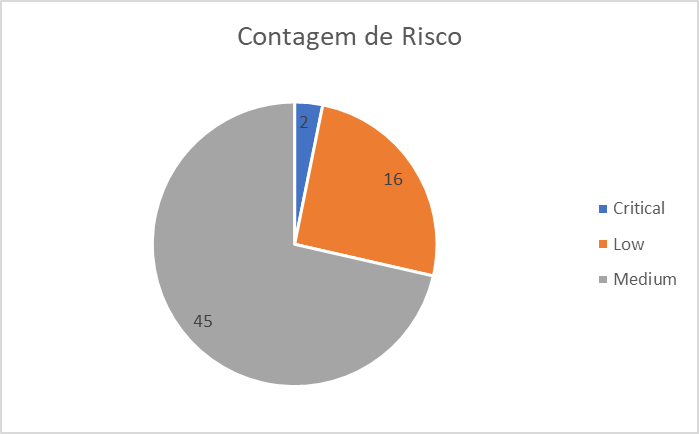
\includegraphics[width=0.7\linewidth]{Imagens/screenshot001}
	\caption[Contagem de Risco]{Contagem de risco dos hosts testados}
	\label{contagem_de_risco}
\end{figure}

\subsection{Alexander Fleming}
\begin{figure}[h]
	\centering
	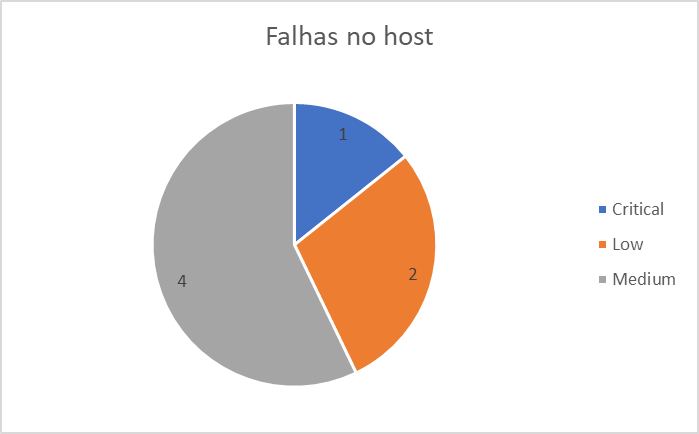
\includegraphics[width=0.7\linewidth]{Imagens/AlexanderFleming}
	\caption[Alexander Fleming]{Contagem de risco do host alexanderfleming.com.br}
	\label{fig:alexanderfleming}
\end{figure}

\subsection{AlphaMU}
\begin{figure}[h]
	\centering
	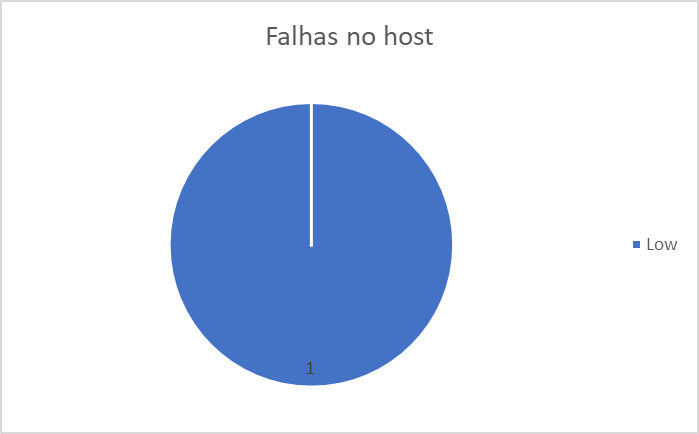
\includegraphics[width=0.7\linewidth]{Imagens/AlphaMU}
	\caption[AlphaMu]{Contagem de risco do host alphamu.com.br}
	\label{fig:alphamu}
\end{figure}

\subsection{Boticario}
\begin{figure}[h]
	\centering
	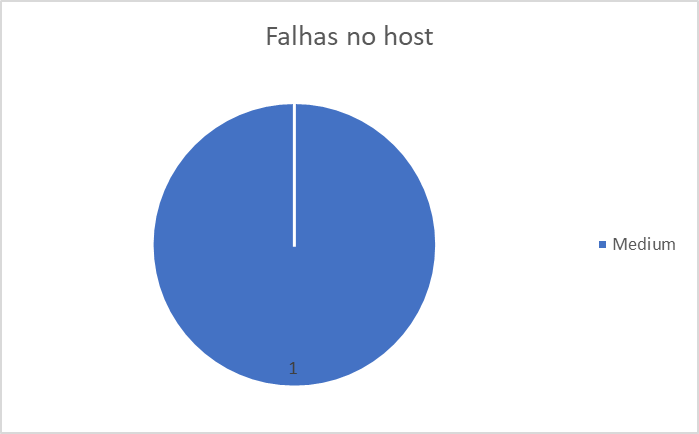
\includegraphics[width=0.7\linewidth]{Imagens/Boticario}
	\caption[Boticario]{Contagem de risco do host boticario.com.br}
	\label{fig:boticario}
\end{figure}

\subsection{Cantina Romana}
\begin{figure}[h]
	\centering
	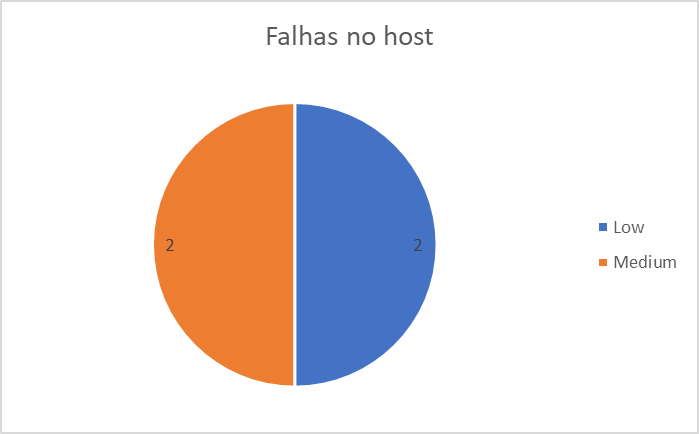
\includegraphics[width=0.7\linewidth]{Imagens/CantinaRomana}
	\caption[Cantina Romana]{Contagem de risco do host cantinaromana.com.br}
	\label{fig:cantinaromana}
\end{figure}

\subsection{Digix}
\begin{figure}[h]
	\centering
	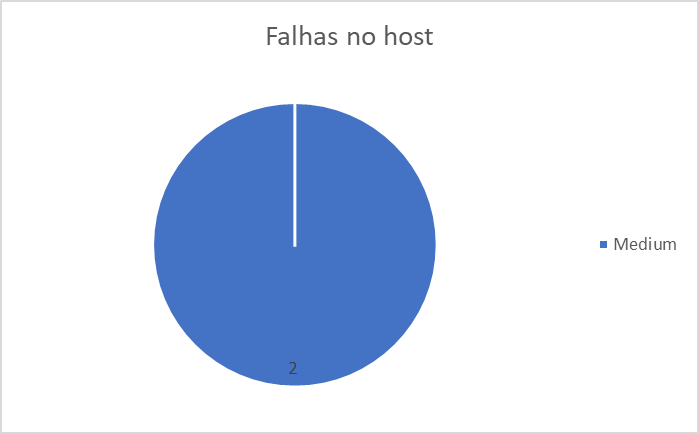
\includegraphics[width=0.7\linewidth]{Imagens/Digix}
	\caption[Digix]{Contagem de risco do host digix.com.br}
	\label{fig:digix}
\end{figure}

\subsection{FACOM, Google e Registro.br}
Não foi encontrada nenhuma falha nos hosts facom.ufms.br, google.com.br e registro.br

\subsection{Jera}
\begin{figure}[h]
	\centering
	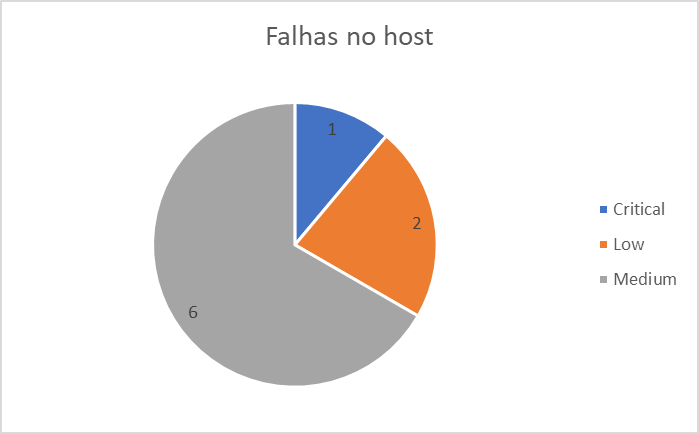
\includegraphics[width=0.7\linewidth]{Imagens/Jera}
	\caption[Jera]{Contagem de risco do host jera.com.br}
	\label{fig:jera}
\end{figure}

\subsection{Locaweb}
\begin{figure}[h]
	\centering
	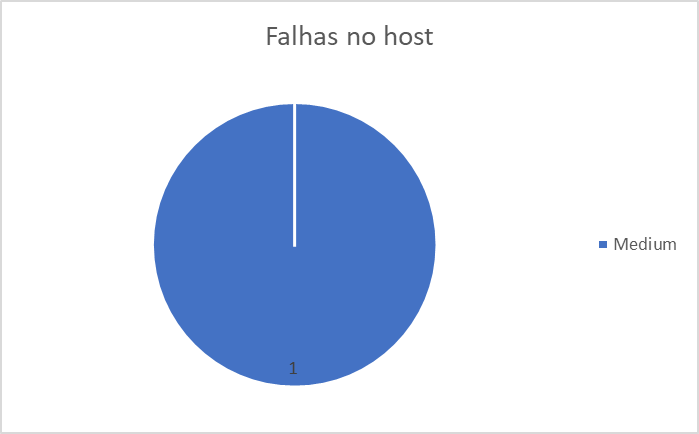
\includegraphics[width=0.7\linewidth]{Imagens/Locaweb}
	\caption[Locaweb]{Contagem de risco do host locaweb.com.br}
	\label{fig:locaweb}
\end{figure}

\subsection{MegaPowerMS}
\begin{figure}[h]
	\centering
	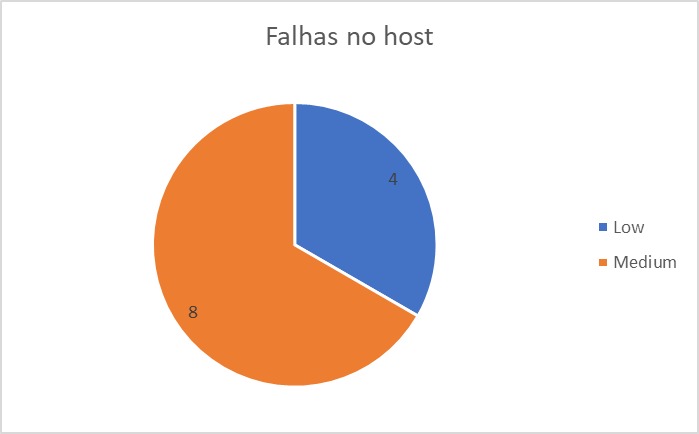
\includegraphics[width=0.7\linewidth]{Imagens/MegaPowerMS}
	\caption[MegaPowerMS]{Contagem de risco do host megapowerms.com.br}
	\label{fig:megapowerms}
\end{figure}

\subsection{Parada Nerd}
\begin{figure}[h]
	\centering
	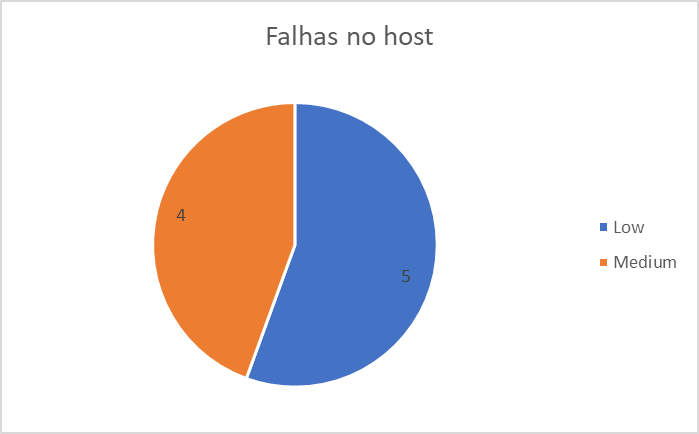
\includegraphics[width=0.7\linewidth]{Imagens/ParadaNerd}
	\caption[Parada Nerd]{Contagem de risco do host paradanerd.com.br}
	\label{fig:paradanerd}
\end{figure}

\subsection{Terra}
\begin{figure}[h]
	\centering
	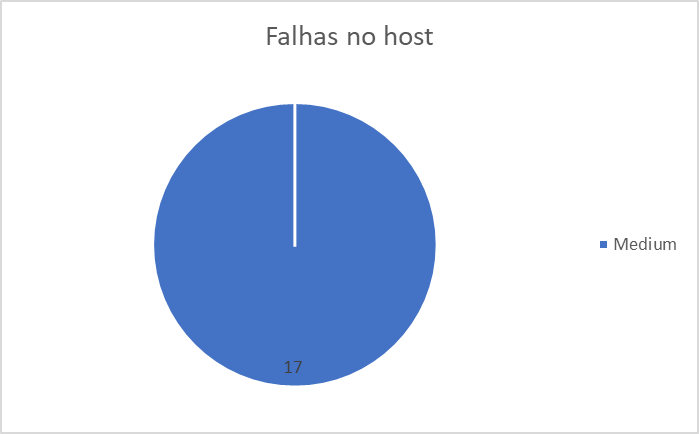
\includegraphics[width=0.7\linewidth]{Imagens/Terra}
	\caption[Terra]{Contagem de risco do host terra.com.br}
	\label{fig:terra}
\end{figure}

\chapter{Comparações}

\chapter{Possíveis soluções para os problemas}

\chapter{Explorando as falhas}

% ----------------------------------------------------------
% Finaliza a parte no bookmark do PDF
% para que se inicie o bookmark na raiz
% e adiciona espaço de parte no Sumário
% ----------------------------------------------------------
\phantompart

% ---
% Conclusão
% ---
\chapter{Conclusão}
% ---

% ----------------------------------------------------------
% ELEMENTOS PÓS-TEXTUAIS
% ----------------------------------------------------------
\postextual
% ----------------------------------------------------------

% ----------------------------------------------------------
% Referências bibliográficas
% ----------------------------------------------------------

%\bibliography{biblio}

%---------------------------------------------------------------------
% INDICE REMISSIVO
%---------------------------------------------------------------------
\phantompart
\printindex
%---------------------------------------------------------------------

\end{document}
